\section{Bäume}
\begin{def*}[note = Wald , index = Wald]
	Ein ungerichteter, einfacher Graph \textbf{ohne Kreise} heisst \textbf{Wald}.
\end{def*}
\begin{def*}[note = Baum , index = Baum]
	Ein Zusammenhängender Wald heisst \textbf{Baum}.
\end{def*}
\begin{def*}[note = Blatt , index = Blatt]
	Ein $v \in V$ mit $\deg(v) = 1$ heisst Blatt.
\end{def*}
\begin{satz*}
	Jeder Baum (mit $|V| \geq 2$) hat mindestens zwei Blätter.
\end{satz*}
\begin{satz*}
	Folgende Aussagen sind äquivalent: $G=(V,E)$ einfacher Graph.
	\begin{enumerate}
		\item $G$ ist ein Baum (zusammenhängend und kreislos)
		\item $G$ ist zusammenhängend, $|V| = |E| + 1$
		\item $G$ ist kreislos, $|V| = |E| + 1$
		\item $G$ ist zusammenhängend, jede $e \in E$ ist Brücke
		\item $G$ kreislos; wird eine zusätzliche Kante eingeführt, erhält $G$ einen Kreis
		\item $\forall u , v \in V$ gibt es genau einen $u$-$v$-Pfad
	\end{enumerate}
	\begin{bew}
		zyklisch: $1 \implies 6 \implies 4 \implies 2 \implies 3 \implies 5 \implies 1$\\
		\begin{tabular}{l p{9cm} }
			$1 \implies 6$	&$G$ zusammenhängend $\implies \exists$ Pfad zwischen beliebigen $u,v$.\\
						&Falls $\exists$ zwei verschiedene $u$-$v$-Pfade, dann hat $G$ einen Kreis \lightning \\
			$6 \implies 4$	&$G$ Zusammenhängend, weil Pfade existieren\\
						&$e$ keine Brücke $\implies$ Zwei verschiedene $u$-$v$-Pfade \lightning \\
			$4 \implies 2$	&Zu zeigen: $|V| = |E| + 1$ Induktion über $|E|$ \\
						&Jede Kante ist Brücke. \\
						&$|E| = |E_1| + |E_2| + 1$ \\
						&Induktionsverankerung: $|E| = 1$ \\
						&Induktionsvoraussetung:\\
						&$|V_1| = |E_1| + 1$ \\
						&$|V_2| = |E_2| + 1$ \\
						&$|V_1| + |V_2| = |E_1| + |E_2| + 2 \implies |V| = |E| + 1$ \\
			$2 \implies 3$	&Annahme: $G$ hat Kreis. Dann $\exists e \in E : (V,E \setminus \{e\})$ zusammenhängend $\implies |V| - (|E| - 1 ) \leq 1 \implies |V| \leq |E|$ \lightning \\
			$3 \implies 5$	&$|V| = |E| + 1$ + Kante $e'$ $\rightsquigarrow E' = E \cup \{e'\}$ \\
						&Immer falls  $|V| \leq |E'|$ : Kreis (heisst $\overline{\deg(v)} \geq 2$) \\
						&$\sum_{v \in V} \deg(v) = 2 |E| \qquad 2|V| = 2|E| \quad |V| = |E|$ \\
						&1. Fall: $\forall v : \deg(v) \geq 2 \implies$ Kreis \\
						&2. Fall: Induktion über $|V|$ Verankerung: $|V| = 1$ $\exists v : \deg(v) \leq 1$ Entferne $v$ und evtl. $e$. Dann $|V \setminus \{v\}| \leq |E' \setminus \{e\} \rightarrow$ Induktionsvoraussetzung: Hat Kreis \\
			$5 \implies 1$	&Zu zeigen: $G$ zusammenhängend\\
						&Annahme: Falls nicht zusammenhängend: Immer noch kreiselos \lightning
		\end{tabular}
		$\blacksquare$
	\end{bew}
\end{satz*}

\subsubsection{Wie viele verschiedene Bäume mit \texorpdfstring{$n$}{n} Knoten gibt es?}
\[
	\begin{matrix*}[l]
		n = 1	& 1	& \text{Linie}		\\
		n = 2	& 1	& \text{Linie}		\\
		n = 3	& 1	& \text{Linie}		\\
		n = 4	& 2	& \text{Linie, Stern}	\\
		n = 5	& 3	& \text{Linie, Stern, Zwischenfall}
	\end{matrix*}
\]
\begin{def*}[note = Spannbaum , index = Spannbaum]
	$G=(V,E)$ zusammenhängend \\
	$H=(V,E')$ ist Spannbaum (spannender Baum), falls
	\begin{itemize}
		\item $H$ ist Baum
		\item $E \subseteq E'$
	\end{itemize}
\end{def*}
\begin{bsp*}
BILD
\end{bsp*}

\subsubsection{Exkurs: Ein wichtiges algorithmisches Problem ist, in einem \textbf{gewichteten Graphen} einen minimalen Spannbaum zu finden.}
\begin{bsp*}[note = ''Gieriger'' Algorithmus]
BILD\\
Gehe die Kanten in aufsteigender Reihenfolge durch unf füge jede Kante hinzu, die keinen Kreis erzeugt.\\
Dann: Es gibt eine optimale Lösung, welche die erste k ''Wahlen'' enthält.\\
Induktion: $k=0 \qquad \checkmark$ \\
$k \rightarrow k+1$: BILD \\
\end{bsp*}

\subsubsection{Markierte Bäume}
Neue Frage: Wie viele Spannbäume hat der $K_n$?\\
$K_n$: Vollständiger Graph mit $n$ Knoten(Clique\index{Clique}(Alle $\binom{n}{2}$ Knotenpaare sind verbunden.))\\
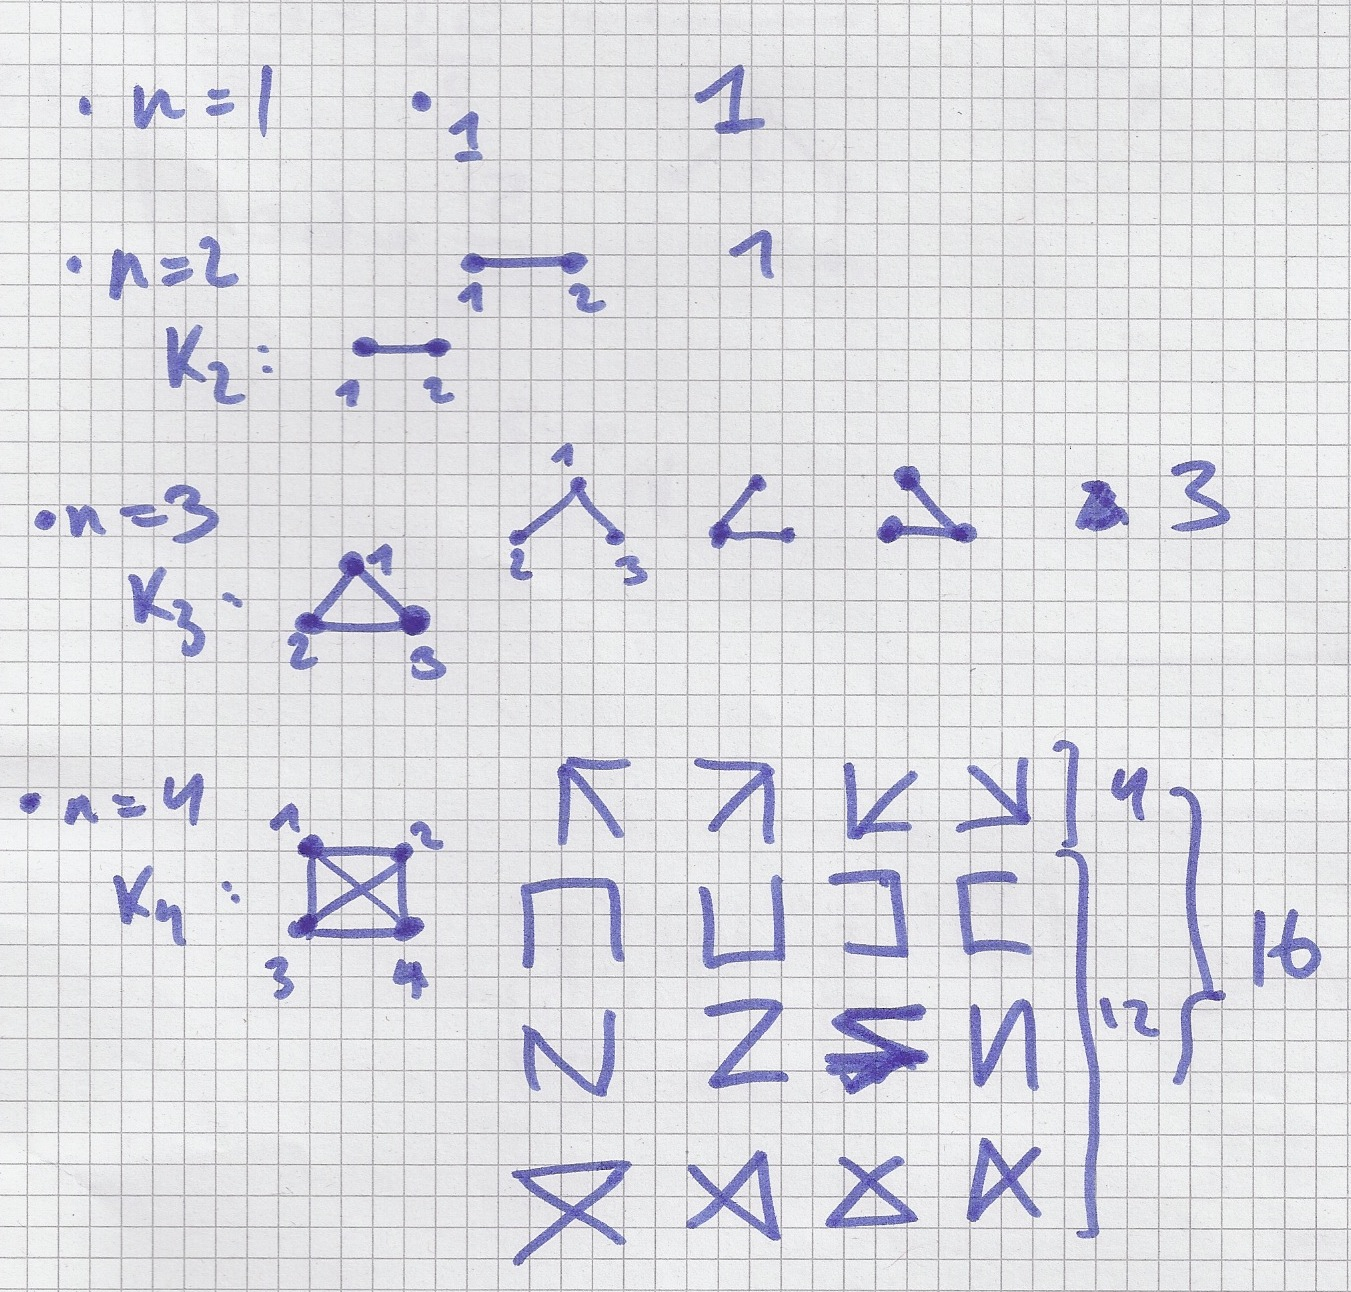
\includegraphics[width=\textwidth]{Bild37} \\
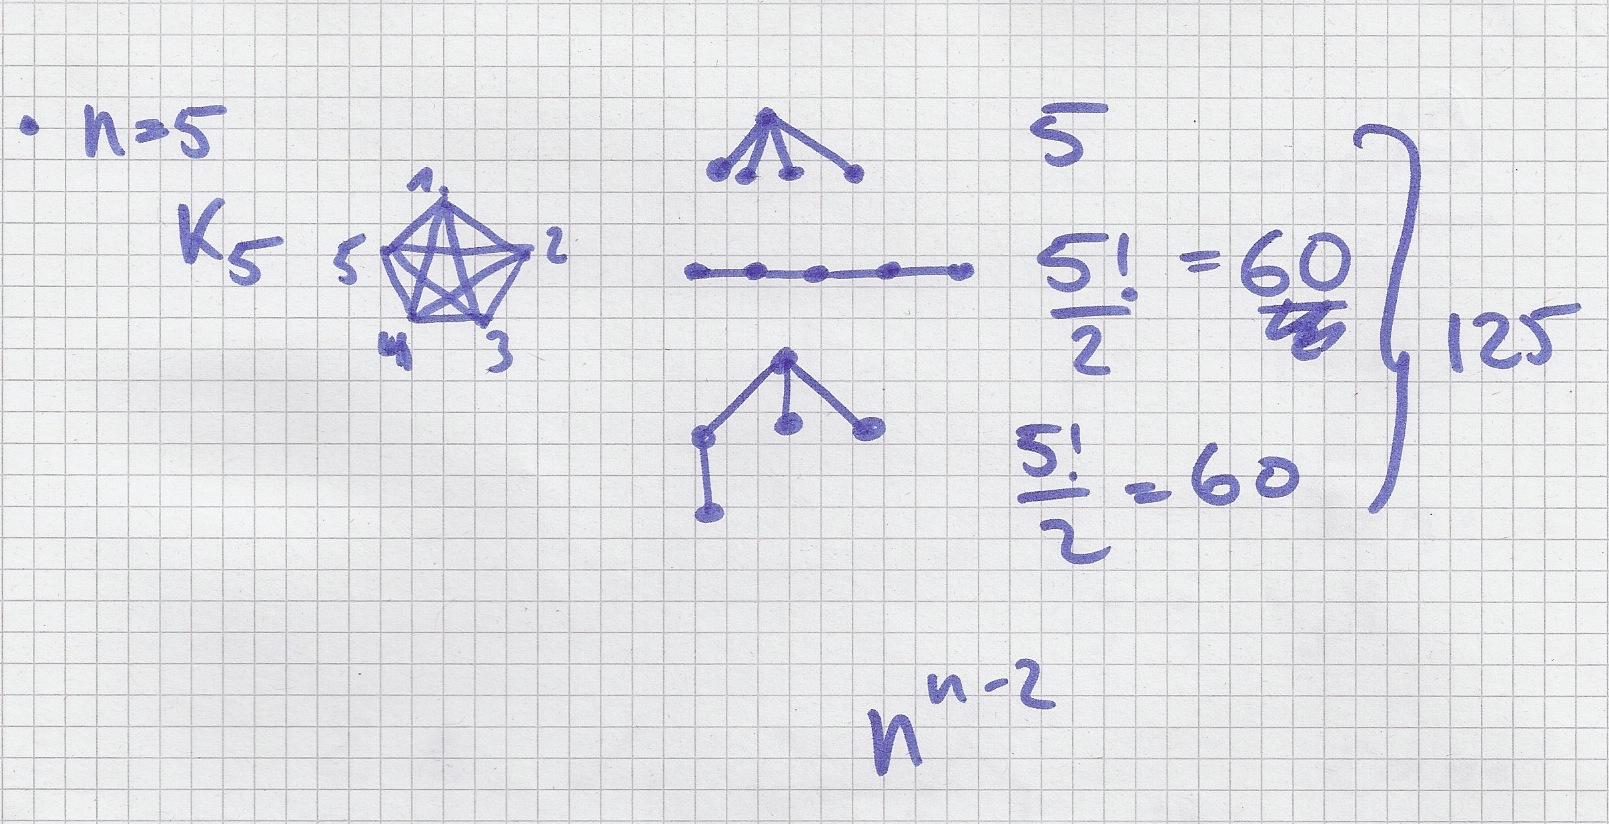
\includegraphics[width=\textwidth]{Bild38}
\begin{def*}[note = isomorph , index = isomorph]
	Zwei Graphen $G=(V,E)$ und $G'=(V',E')$ sind \textbf{isomorph}, $G \cong G'$ falls $\exists f: V \rightarrow V'$ bijektiv so, dass $\forall v,w \in V : (v,w) \in E \iff (f(v),f(w)) \in E'$
\end{def*}
\begin{bsp*}
	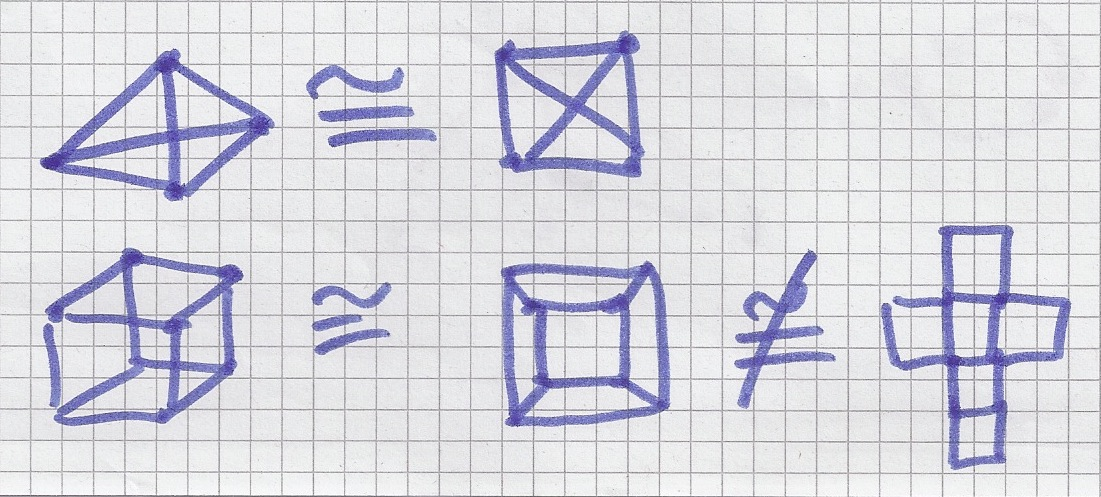
\includegraphics[width=\textwidth]{Bild39}
\end{bsp*}
\begin{satz*}[note = (Cayley)]
	Die Anzahl markierter Bäume mit $n$ Knoten ist $n^{n-2}$
	\begin{bew}
		Wir zählen markierte Bäume mit zwei Zusatzmarkierungen O $\square$, beide beliebig gesetzt.\\
		\begin{bsp*}
			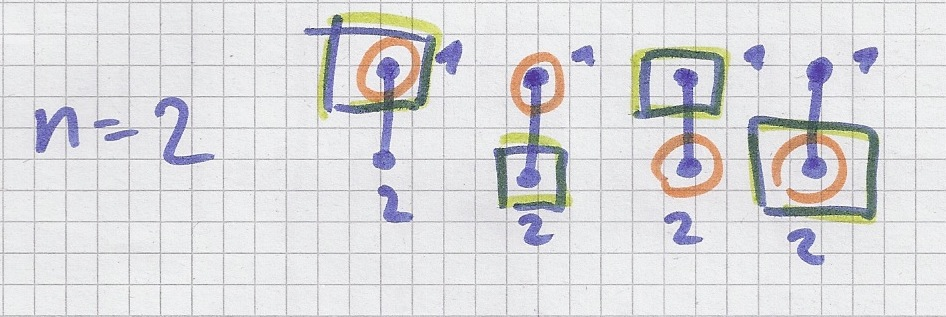
\includegraphics[width=\textwidth]{Bild40}
		\end{bsp*}
		Wir zeigen: von diesen gibt es genau $n^n$.\\
		Bijektion mit $\{f: \{1, \dotsc , n \} \rightarrow \{1, \dotsc , n \} \}$\\
		$\abs{\{\dots\}} = n^n$\\
		$f \mapsto$ markierter Baum mit O $\square$\\
		\[ f = \begin{pmatrix}
			1	&2	&3	&4	&5	&6	&7	&8	&9	&10	\\
			7	&5	&5	&9	&1	&2	&5	&8	&4	&7	
		\end{pmatrix} \]
		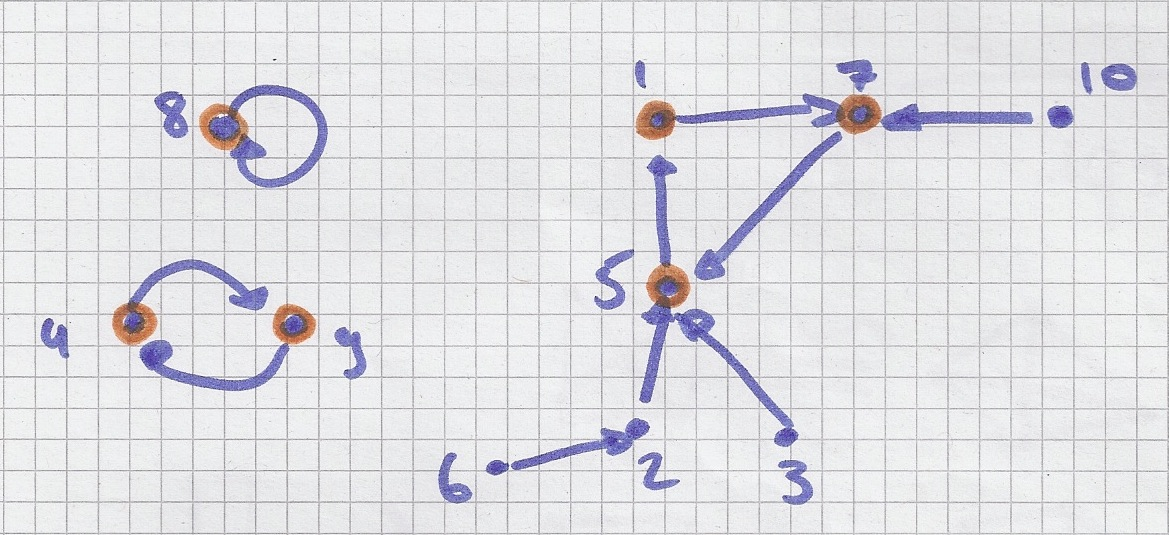
\includegraphics[width=\textwidth]{Bild41} \\
		In jeder Zusammenhangskomponente gibt es einen Zyklus.\\
		Eingeschränkt auf die Knoten M in den Zyklen ist $f$ Bijektion (Permutation)\\
		\[ f|M = \begin{pmatrix}
			1	&4	&5	&7	&8	&9	\\
			7	&9	&1	&5	&8	&4	
		\end{pmatrix} \qquad \text{''eingeschränkt auf''} \]
		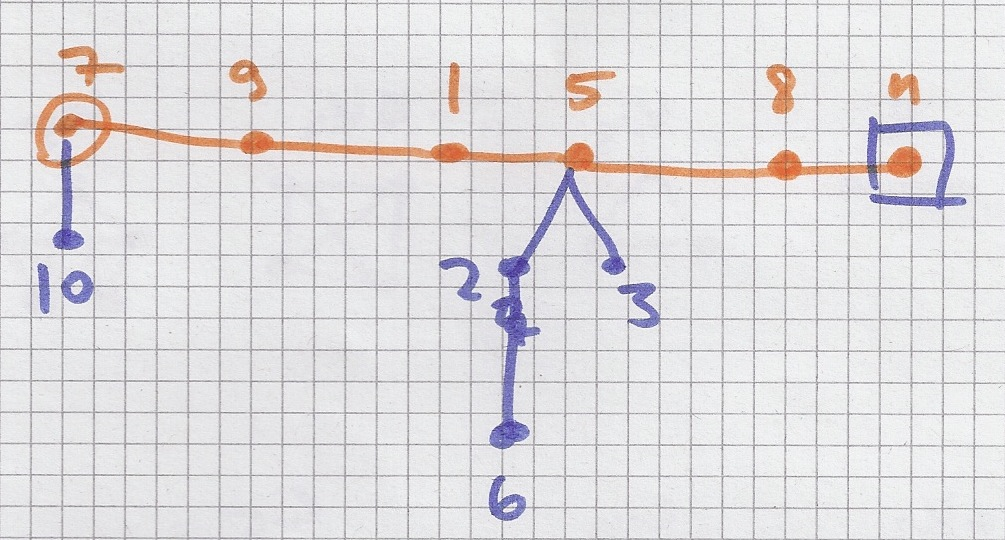
\includegraphics[width=\textwidth]{Bild42}
	\end{bew}
	\begin{bew}[head = Beweis der Umkehrrichtung:]
		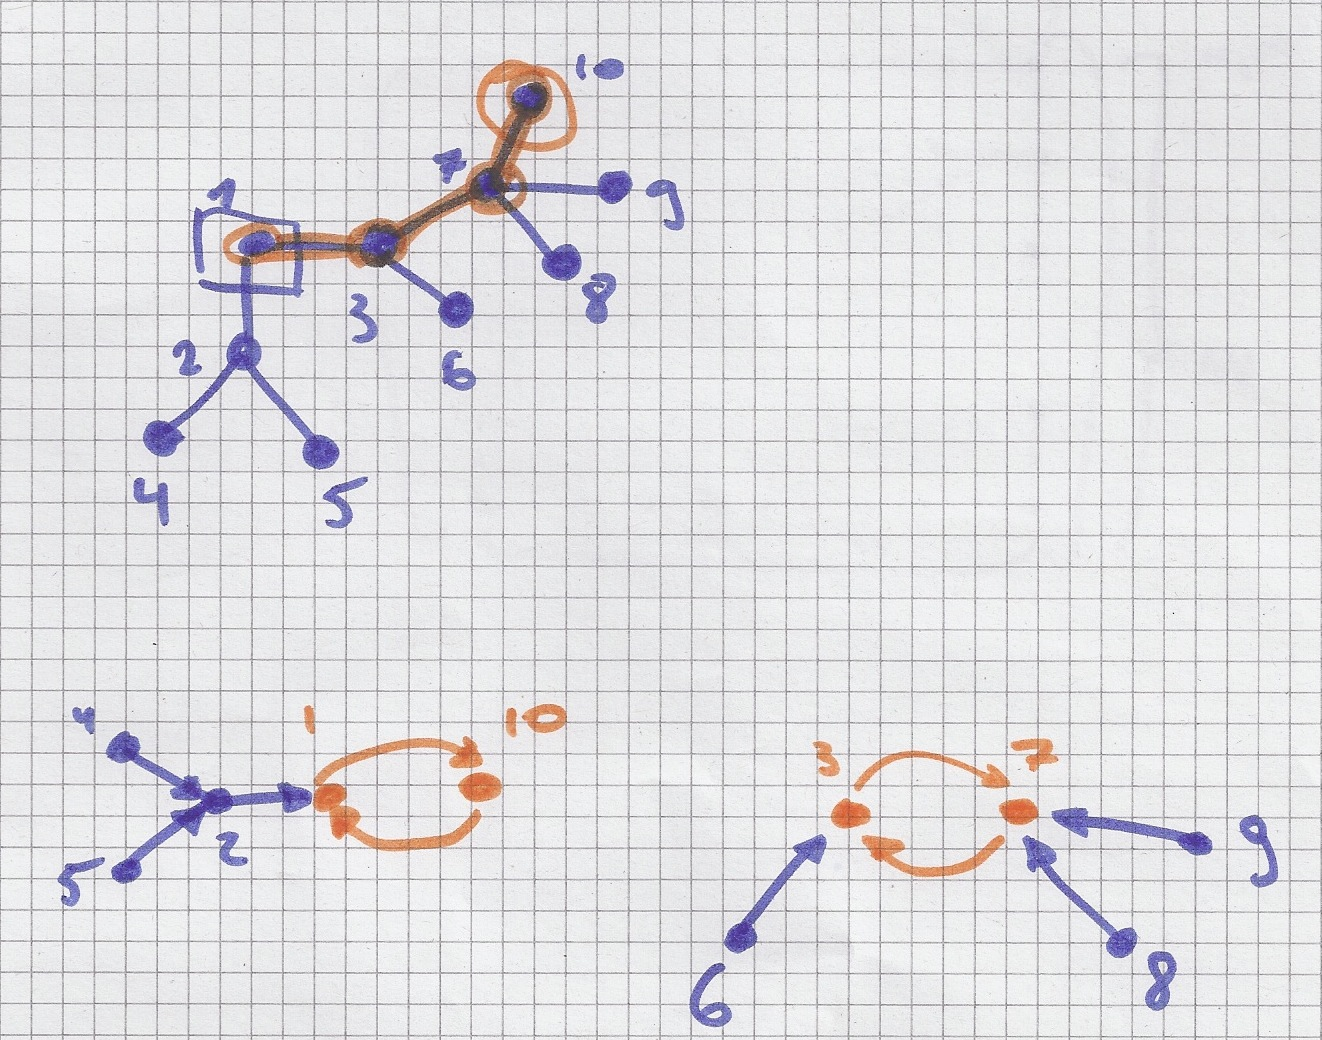
\includegraphics[width=\textwidth]{Bild43}
		\begin{gather*}
			f|M = \begin{pmatrix}
				1	&3	&7	&10	\\
				10	&7	&3	&1	
			\end{pmatrix}\\
			f = \begin{pmatrix}
				1	&2	&3	&4	&5	&6	&7	&8	&9	&10	\\
				10	&1	&7	&2	&2	&3	&3	&7	&7	&1	
			\end{pmatrix}\\
			\blacksquare
		\end{gather*}
	\end{bew}
\end{satz*}
